%\subsection{Eigenspace Overlap}
%\label{subsec:eigen_overlap}
%	\begin{itemize}
%		\item Introduce the eigenspace overlap metric.
%%		\item Present the generalization bound.
%	\end{itemize}
%	
%\subsection{Generalization of Compressed Embeddings}
%\label{subsec:revisit}
%	\begin{itemize}
%		\item Empirically demonstrate the correlation with respect to generalization performance
%		\item Discuss why it explains better than Deltas (if have not discuss the relation to Deltas, we should discuss here also).
%	\end{itemize}


In this section, we introduce the \textit{eigenspace overlap metric} to measure the quality of a compressed embedding relative to the uncompressed embedding.
We prove average-case generalization bounds for this metric in the context of linear regression, and show that this metric indeed aligns very well with the downstream performance of the compressed embeddings.

\subsection{Eigenspace Overlap and Generalization}
\label{subsec:eigen_overlap}
\begin{definition}
Given two embedding matrices $X \in \RR^{n \times d}$, $\tX \in \RR^{n \times k}$, whose Gram matrices have eigendecompositions $XX^T = USU^T$, $\tX\tX^T = VRV^T$ for $U \in \RR^{n\times d}$, $V\in \RR^{n \times k}$, we define the eigenspace overlap metric $\eigover(X,\tX) \defeq  \frac{1}{\max(d,k)}\|U^T V\|_F^2$.\footnote{We normalize by $\max(d,k)$ in order}
\end{definition}

This metric measures the degree to which the span of the eigenvectors with nonzero eigenvalue of $\tX\tX^T$ agrees with that of $XX^T$.
In particular, assuming $k\leq d$, it measures the ratio between the squared Frobenius norm of $U$ before and after being projected onto $V$.
As an example, if the span $\Span(V)$ of the columns of $V$ is a subspace of $\Span(U)$, then $\eigover(X,\tX) = \frac{1}{d}\|U^T V\|_F^2 = \frac{1}{d}\|UU^T V\|_F^2 = \frac{1}{d}\|V\|_F^2 = \frac{k}{d}$.
In contrast, if $\Span(V)$ is orthogonal to $\Span(U)$, then $\eigover(X,\tX) = 0$.

We now show that this metric is closely related to the generalization performance of the linear regression model trained using the compressed embeddings $\tX$ in place of $X$.
For simplicity, we will consider here the noiseless fixed design regression setting;
In this setting, the training loss is equal to the generalization loss.
Letting $y\in\RR^n$ denote the vector of labels and using the closed form solution for the optimal parameters $w^* = (X^T X)^{-1}X^Ty$, we can see that the generalization performance is equal to $\cR(X) = \|Xw^* - y\|^2 = \|y\|^2 - \|U^T y\|^2$ (derivation in Appendix \todo{XX}).

To expose the influence of the eigenspace overlap on the generalation performance, it will be necessary for us to considering an average-case analysis.
This is necessary because in worst-case analysis, if there exists a single direction in $\Span(U)$ orthogonal to $\Span(V)$ (which always occurs when $\dim(V) < \dim(U)$) the label vector $y$ can simply be equal to this direction.
In this case $\cR(X) = \|y\|^2 - \|U^T y\|^2 = 0$, while $\cR(\tX) = \|y\|^2 - \|V^T y\|^2 = \|y\|^2$.
Thus, the setting we will consider instead is one where $y$ is a random vector in $\Span(U)$.
We consider this setting for simplicity because we are most interested in the situation where we know the uncompressed embedding matrix $X$ performs well \todo{might want to explain why y in span of U means performing well.}, and we would like to understand how well $\tX$ will do.
We now present our average-case result:

\begin{proposition}
If $y = Uz$ for a random vector $z \in \RR^d$ with zero mean and identity covariance, then
\begin{eqnarray}
\expect{y}{\cR(\tX) - \cR(X)} &=& d\cdot(1 - \eigover(X,\tX))
\end{eqnarray}
\end{proposition}

This proposition reveals that a larger eigenspace overlap value results in better generalization performance for the compressed embedding.

\subsection{Revisit Performance of Compressed Embeddings}
\label{subsec:revisit}
We now demonstrate that unlike the metrics we discussed in Section~\ref{sec:background}, this metric empirically aligns very well with the performance of compressed embeddings on downstream tasks.
In Figure~\ref{fig:good_correlation} we show scatter plots of downstream performance vs.\ eigenspace overlap, and see that in general higher eigenspace overlap corresponds to better performance.
Thus, even though our analysis is for a linear regression setting, we can see that this metric predicts performance well on a variety of downstream tasks which use neural networks for training.

\todo{Discuss performance relative to $\Delta_1$,$\Delta_2$?}

\begin{figure*}
	\begin{tabular}{@{\hskip -0.0in}c@{\hskip -0.0in}c@{\hskip -0.0in}c@{\hskip -0.0in}c@{\hskip -0.0in}}
		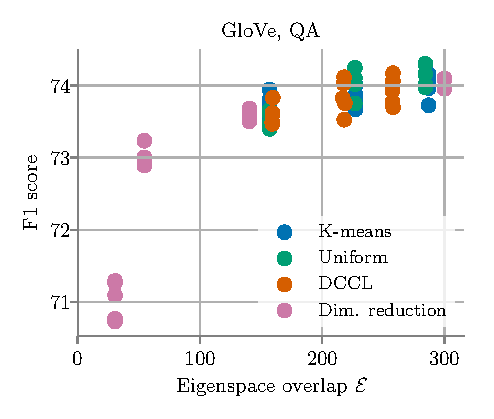
\includegraphics[width=.245\linewidth]{figures/glove400k_qa_best-f1_vs_subspace-eig-overlap_linx.pdf} &
		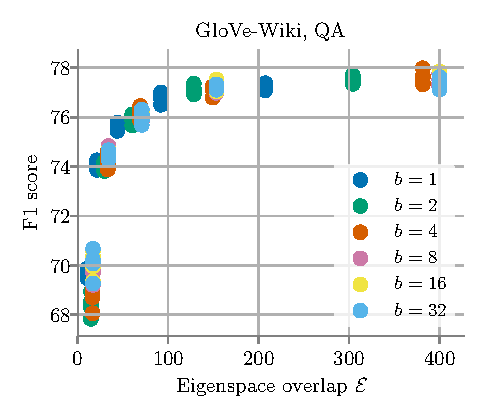
\includegraphics[width=.245\linewidth]{figures/glove-wiki400k-am_qa_best-f1_vs_subspace-eig-overlap_linx.pdf} &
		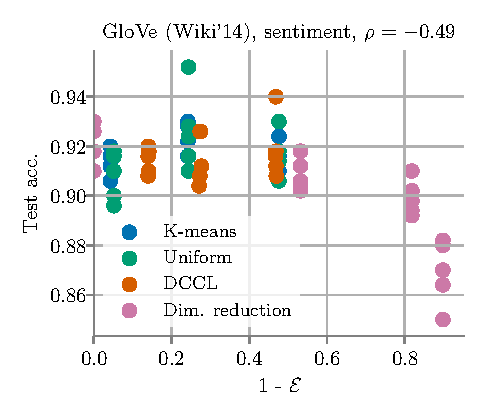
\includegraphics[width=.245\linewidth]{figures/glove400k_sentiment_trec_test-acc_vs_subspace-eig-overlap_linx.pdf} &
		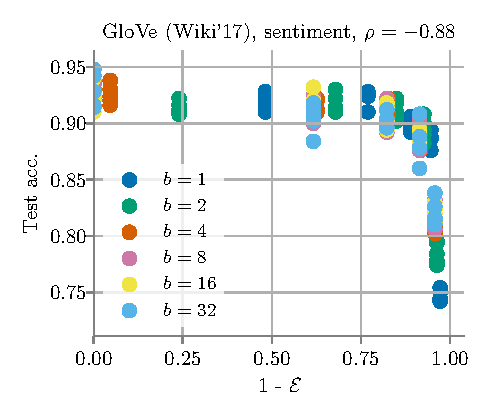
\includegraphics[width=.245\linewidth]{figures/glove-wiki400k-am_sentiment_trec_test-acc_vs_subspace-eig-overlap_linx.pdf}	\\
		(a) GloVe, QA & (b) GloVe Wiki, QA  & (c) GloVe, sentiment & (d) GloVe Wiki, sentiment
	\end{tabular}
	\label{fig:good_correlation}
	\caption{Our proposed compression quality metric eigenspace overlap correlates strongly with the downstream task performance of compressed embeddings. \todo{explain what does adaptive-det mean?} On both the question answering and sentiment analysis task, we demonstrate that eigenspace overlap consistently achieves strong correlation 1) across different compression methods (shown in (a), (c)) and 2) across different precision for the uniform quantization methods (shown in (b), (d)). In other words, embeddings compressed by different methods using different configurations can performs similarly in downstream tasks, when they have similar eigenspace overlap with the same reference uncompressed embedding.}
\end{figure*}
